\documentclass[12pt]{article}

% ============================================================
% IDIOMA Y CODIFICACIÓN
% ============================================================
\usepackage[spanish, es-noshorthands]{babel}
\usepackage[utf8]{inputenc}
\usepackage[T1]{fontenc}

% ============================================================
% COLOR
% ============================================================
\usepackage[dvipsnames]{xcolor}

% ============================================================
% MÁRGENES Y GEOMETRÍA
% ============================================================
\usepackage[a4paper, margin=2.5cm]{geometry}

% ============================================================
% ESPACIADO MEJORADO
% ============================================================
\usepackage{setspace}
\setstretch{1.15}

\setlength{\parskip}{0.5em}
\setlength{\parindent}{0pt}

% ============================================================
% TIPOGRAFÍA
% ============================================================
\usepackage{lmodern}

% ============================================================
% FORMATO DE TÍTULOS
% ============================================================
\usepackage{titlesec}

\titleformat{\section}
  {\Large\bfseries}
  {\thesection.}
  {0.5em}
  {}

\titlespacing*{\section}{0pt}{1.5em}{0.8em}

% ============================================================
% MATEMÁTICAS
% ============================================================
\usepackage{amsmath, amssymb, amsfonts}

% ============================================================
% CÓDIGO FUENTE
% ============================================================
\usepackage{listings}

% ============================================================
% GRÁFICOS
% ============================================================
\usepackage{graphicx}
\usepackage{float}
\usepackage{tikz}
\usetikzlibrary{arrows.meta}

% ============================================================
% TABLAS
% ============================================================
\usepackage{booktabs}
\usepackage{array}
\usepackage{multirow}

\definecolor{codebg}{RGB}{248, 248, 248}
\definecolor{codeframe}{RGB}{200, 200, 200}
\definecolor{codecomment}{RGB}{106, 153, 85}
\definecolor{codekeyword}{RGB}{86, 156, 214}
\definecolor{codestring}{RGB}{206, 145, 120}
\definecolor{codenumber}{RGB}{181, 206, 168}

\lstdefinestyle{estilo_base}{
    backgroundcolor=\color{codebg},
    frame=single,
    rulecolor=\color{codeframe},
    basicstyle=\ttfamily\small,
    commentstyle=\color{codecomment}\itshape,
    keywordstyle=\color{codekeyword}\bfseries,
    stringstyle=\color{codestring},
    numberstyle=\tiny\color{codenumber},
    numbers=left,
    numbersep=8pt,
    breaklines=true,
    breakatwhitespace=true,
    tabsize=4,
    showstringspaces=false,
    captionpos=b,
    literate=
        {á}{{\'a}}1 {é}{{\'e}}1 {í}{{\'i}}1 {ó}{{\'o}}1 {ú}{{\'u}}1
        {Á}{{\'A}}1 {É}{{\'E}}1 {Í}{{\'I}}1 {Ó}{{\'O}}1 {Ú}{{\'U}}1
        {ñ}{{\~n}}1 {Ñ}{{\~N}}1 {ü}{{\"u}}1 {¿}{{?`}}1 {¡}{{!`}}1,
}

\newcommand{\codigo}[1]{\texttt{\small #1}}

% ============================================================
% LISTAS Y NUMERACIÓN
% ============================================================
\usepackage{enumitem}

% ============================================================
% ENLACES E HIPERTEXTO
% ============================================================
\usepackage{hyperref}
\hypersetup{
    colorlinks  = true,
    linkcolor   = black,
    urlcolor    = blue!60!black,
    citecolor   = black,
    pdftitle    = {Cálculo Diferencial e Integral I - Trabajo Práctico N° 2 - Parte 2},
    pdfauthor   = {Facundo Luna},
}

% ============================================================
% ENCABEZADO Y PIE DE PÁGINA
% ============================================================
\usepackage{fancyhdr}
\pagestyle{fancy}
\fancyhf{}
\renewcommand{\headrulewidth}{0.4pt}
\renewcommand{\footrulewidth}{0.4pt}
\fancyhead[L]{\small Cálculo Diferencial e Integral I}
\fancyhead[R]{\small Trabajo Práctico N° 2 - Parte 2}
\fancyfoot[L]{\small Facundo Luna}
\fancyfoot[R]{\small \thepage}

% ============================================================
% DATOS DEL TRABAJO
% ============================================================

\newcommand{\universidad}{Universidad Católica de Salta}
\newcommand{\carrera}{Licenciatura en Ciencia de Datos}
\newcommand{\materia}{Cálculo Diferencial e Integral I}
\newcommand{\trabajo}{Trabajo Práctico N° 2 - Parte 2}
\newcommand{\profesor}{Lic. Mauro Vaca}
\newcommand{\alumno}{Facundo Luna}
\newcommand{\fecha}{\today}

\newcommand{\logoincluido}{%
    
\includegraphics[width=3.5cm]{../../../assets/ucasal-logo.png}\\[0.5cm]%
}
\newcommand{\logoomitido}{\vspace{1cm}}
\newcommand{\logoportada}{\logoincluido}

% ============================================================
% COMANDO SOLUCIÓN
% ============================================================
\newcommand{\solucion}{%
    \vspace{0.8em}%
    \textbf{Solución:}%
}

% ============================================================
% COMANDO VOLVER AL ÍNDICE
% ============================================================
\newcommand{\volverindice}{%
    \vspace{1em}%
    \begin{flushright}%
        \hyperlink{indice}{\small $\uparrow$ Volver al índice}%
    \end{flushright}%
}

% ============================================================

\begin{document}

% ======================== PORTADA ===========================

\begin{titlepage}
    \centering

    \logoportada

    \rule{\linewidth}{1.5pt}\\[0.4cm]

    {\large\scshape \universidad}\\[0.2cm]
    {\large \carrera}\\[0.1cm]

    \rule{\linewidth}{0.5pt}\\[1.5cm]

    {\Huge\bfseries \trabajo}\\[0.8cm]
    {\LARGE \materia}\\[2cm]

    \begin{tabular}{rl}
        \textbf{Alumno:}   & \alumno   \\[0.3cm]
        \textbf{Profesor:} & \profesor \\[0.3cm]
        \textbf{Fecha:}    & \fecha    \\
    \end{tabular}

    \vfill

    \rule{\linewidth}{1.5pt}

\end{titlepage}

% ======================== ÍNDICE ============================

\newpage
\tableofcontents
\hypertarget{indice}{}
\setcounter{tocdepth}{2}

% ======================== ACTIVIDADES =======================

% ======================== ACTIVIDAD 9 ========================
\newpage
\section[Discontinuidades]{A partir de la gráfica de $f$, establezca el número en el cual $f$ es discontinua y explique por qué. Clasifique las discontinuidades.}
 
\begin{enumerate}[label=\alph*.-]
 
    % ======================== item a ========================
    \item A partir de la gráfica de $f$, establezca el número en el cual $f$ es discontinua y explique por qué. Clasifique las discontinuidades.
 
    \begin{figure}[h]
    \centering
    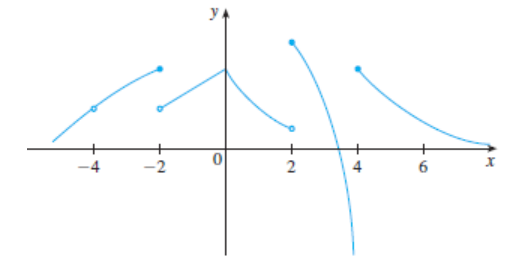
\includegraphics[width=0.6\textwidth]{assets/9_a.png}
    \caption{Gráfica de f}
    \label{fig:grafica de f}
    \end{figure}
 
    \solucion
 
    \vspace{0.5em}
    \textbf{Recordatorio de clasificación:}
 
    \begin{itemize}[leftmargin=2em]
        \item \textbf{Evitable:} $\exists \lim_{x \to a} f(x)$ pero $\nexists f(a)$, o bien $\lim_{x \to a} f(x) \neq f(a)$.
        \item \textbf{No Evitable — salto finito:} $\nexists \lim_{x \to a} f(x)$, los límites laterales $\ell_i$ y $\ell_d$ existen pero $\ell_i \neq \ell_d$.
        \item \textbf{No Evitable — salto infinito:} $\nexists \lim_{x \to a} f(x)$ porque al menos uno de los límites laterales es $\pm\infty$.
    \end{itemize}

    $f$ es discontinua en los siguientes puntos:
 
    \textbf{$x = -4$:} La función no está definida en este punto, es decir, $x = -4$ no pertenece al dominio de $f$. En cuanto al tipo de discontinuidad, es una \textbf{discontinuidad evitable}.
 
    \textbf{$x = -2$:} $f$ es discontinua en este punto porque, si bien la función está definida en $x = -2$, el límite no existe debido a que los límites laterales por izquierda y derecha son distintos. Luego, en cuanto a su tipo de discontinuidad, es una \textbf{discontinuidad No Evitable de salto finito}.
 
    \textbf{$x = 2$:} De manera análoga al caso anterior, la función está definida en $x = 2$ pero el límite en ese punto no existe. La discontinuidad es \textbf{No Evitable de salto finito}.
 
    \textbf{$x = 4$:} En este punto la función es discontinua, porque si bien está definida en $x = 4$, el límite no existe. Se observa que al acercarnos a $4$ por izquierda la función tiende a $-\infty$, mientras que al aproximarnos a $x = 4$ por derecha el valor del límite es un número finito $\neq 0$. La discontinuidad es \textbf{No Evitable de salto infinito}.
 
    \vspace{0.5em}
    \textbf{Resumen de clasificación:}
 
    \begin{center}
    \begin{tabular}{cll}
        \toprule
        Punto & Tipo & Subtipo \\
        \midrule
        $x = -4$ & Evitable & --- \\
        $x = -2$ & No Evitable & Salto finito \\
        $x = 2$  & No Evitable & Salto finito \\
        $x = 4$  & No Evitable & Salto infinito \\
        \bottomrule
    \end{tabular}
    \end{center}
 
    \newpage
    % ======================== item b ========================
    \item Para cada uno de los números que se obtuvieron en el inciso a), determine si $f$ es continua por la derecha, por la izquierda o por ninguno de los dos lados.
 
    \solucion
 
    Recordemos las definiciones:
    \begin{itemize}[leftmargin=2em]
        \item $f$ es \textbf{continua por la izquierda} en $a$ si: $\displaystyle\lim_{x \to a^-} f(x) = f(a)$
        \item $f$ es \textbf{continua por la derecha} en $a$ si: $\displaystyle\lim_{x \to a^+} f(x) = f(a)$
    \end{itemize}
 
    Los puntos obtenidos son: $x_1 = -4$, $x_2 = -2$, $x_3 = 2$, $x_4 = 4$.
 
    \vspace{0.5em}
    \textbf{i) Analizamos el punto $x_1 = -4$:}
 
    Observando la gráfica:
    \[
    \lim_{x \to -4^-} f(x) = \ell_1 \quad \text{(existe y es finito)}
    \]
    \[
    \lim_{x \to -4^+} f(x) = \ell_2 \quad \text{(existe y es finito} \text{)}
    \]
    
    Además, $f(-4)$ no está definida (hay un círculo vacío en la gráfica).
    
    Como ambos límites laterales existen y son finitos, $f$ es \textbf{continua por la izquierda y continua por la derecha} en $x = -4$.
    
    La discontinuidad es evitable porque ambos límites laterales son finitos.
 
    \vspace{0.5em}
    \textbf{ii) Analizamos el punto $x_2 = -2$:}
 
    Observando la gráfica:
    \[
    \lim_{x \to -2^-} f(x) = \ell_1 \quad \text{(existe y es finito)}
    \]
    \[
    \lim_{x \to -2^+} f(x) = \ell_2 \quad \text{(existe y es finito, pero } \ell_1 \neq \ell_2\text{)}
    \]
    
    Además, $f(-2) = 0$ existe, la función esta definida en ese punto.
    
    Como el límite lateral por izquierda existe y es igual al valor de la función en este punto, $f$ es \textbf{continua por la izquierda} en $x = -2$.
    
    La discontinuidad es no evitable de salto finito porque los límites laterales son diferentes.
 
    \newpage
    \vspace{0.5em}
    \textbf{iii) Analizamos el punto $x_3 = 2$:}
 
    Observando la gráfica:
    \[
    \lim_{x \to 2^-} f(x) = \ell_1 \quad \text{(existe y es finito)} \lim_{x \to 2^+} f(x) = \quad \text{(existe y es finito)}
    \]
    
    Como el límite lateral por derecha existe y es igual al valor de la función en este punto, $f$ es \textbf{continua por la derecha} en $x = 2$.
    
    La discontinuidad es no evitable de salto finito.
 
    \vspace{0.5em}
    \textbf{iv) Analizamos el punto $x_4 = 4$:}
 
    Observando la gráfica:
    \[
    \lim_{x \to 4^-} f(x) = -\infty \qquad \lim_{x \to 4^+} f(x) = \ell \quad \text{(existe y es finito)}
    \]
    
    Como el límite por la izquierda es infinito pero el límite por la derecha es finito, $f$ \textbf{no es continua por la izquierda, pero sí es continua por la derecha} en $x = 4$.
    
    La discontinuidad es no evitable de salto infinito.
 
    \newpage
    % ======================== item c ========================
    \item A partir de la gráfica de $g$, establezca los intervalos sobre los que es continua.
 
    \begin{figure}[h]
    \centering
    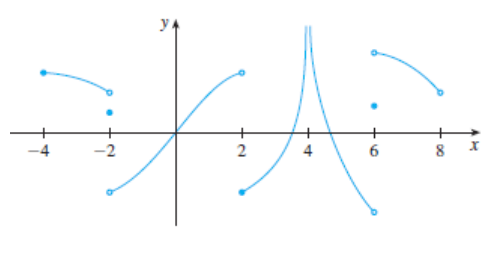
\includegraphics[width=0.6\textwidth]{assets/9_c.png}
    \caption{Gráfico de g}
    \label{fig:grafica de g}
    \end{figure}
 
    \solucion
 
    A partir de la gráfica de $g$, identificamos los puntos de discontinuidad: $x = -2$, $x = 2$, $x = 4$, $x = 6$, $x = 8$.
 
    En consecuencia, los intervalos sobre los que $g$ es continua son:
 
    \[
    \boxed{(-4,\ -2) \cup (-2,\ 2) \cup [2,\ 4) \cup (4,\ 6) \cup (6,\ 8)}
    \]
 
\end{enumerate}
 
\volverindice
\newpage

% ======================== ACTIVIDAD 10 ========================
\newpage
\section[Continuidad en un número]{Utilice la definición de continuidad y las propiedades de los límites para demostrar que cada una de las siguientes funciones es continua.}

\begin{enumerate}[label=\alph*.-]

    % ======================== item a ========================
    \item
    \solucion

    Una función $f$ es continua en un número $x = a$ si:
    \[
    \lim_{x \to a} f(x) = f(a)
    \]

    Esto implica lo siguiente:
    \begin{enumerate}[label=\arabic*.-]
        \item $f(a)$ está definida ($a$ pertenece al dominio de $f$)
        \item $\displaystyle\lim_{x \to a} f(x)$ existe
        \item $\displaystyle\lim_{x \to a} f(x) = f(a)$
    \end{enumerate}

    \begin{enumerate}[label=\roman*.]

        % ---------- i ----------
        \item $f(x) = \dfrac{2x+3}{x-2}$ \quad $a = -1$

        \textbf{1.} Evaluamos $f(-1)$:
        \[
        f(-1) = \frac{2(-1)+3}{-1-2} = \frac{-2+3}{-3} = \frac{1}{-3} = -\frac{1}{3}
        \]

        \textbf{2 y 3.} Calculamos el límite aplicando propiedades (sustitución directa, ya que $x = -1$ no anula el denominador):
        \[
        \lim_{x \to -1} \left(\frac{2x+3}{x-2}\right) = \frac{2(-1)+3}{-1-2} = \frac{1}{-3} = -\frac{1}{3}
        \]

        Debido a que $\displaystyle\lim_{x \to -1} f(x) = f(-1) = -\dfrac{1}{3}$, $f$ es continua en $x = -1$.

        \vspace{0.5em}
        % ---------- ii ----------
        \item $g(x) = \dfrac{2x - 3x^2}{1 + x^3}$ \quad $a = 1$

        \textbf{1.} Evaluamos $g(1)$:
        \[
        g(1) = \frac{2(1) - 3(1)^2}{1 + (1)^3} = \frac{2 - 3}{1 + 1} = \frac{-1}{2} = -\frac{1}{2}
        \]

        \textbf{2 y 3.} Calculamos el límite (sustitución directa, ya que $x = 1$ no anula el denominador pues $1 + 1^3 = 2 \neq 0$):
        \[
        \lim_{x \to 1} \left(\frac{2x - 3x^2}{1 + x^3}\right) = \frac{2(1) - 3(1)^2}{1 + (1)^3} = \frac{2 - 3}{2} = -\frac{1}{2}
        \]

        Luego, debido a que $\displaystyle\lim_{x \to 1} g(x) = g(1) = -\dfrac{1}{2}$, se tiene que la función $g$ es continua en $x = 1$.

    \end{enumerate}

    % ======================== item b ========================
    \item
    \solucion

    Una función $f$ es continua en un intervalo cerrado $[a, b]$ si es continua en el intervalo abierto $(a, b)$ y además:
    \[
    \lim_{x \to a^+} f(x) = f(a) \qquad \text{y} \qquad \lim_{x \to b^-} f(x) = f(b)
    \]

    \begin{enumerate}[label=\roman*.]

        % ---------- i ----------
        \item $f(x) = \dfrac{2x+3}{x-2}$ \quad $(2,\ \infty)$

        El punto $x = 2$ anula el denominador, por lo que $x = 2 \notin (2, \infty)$: no pertenece al intervalo. Tomamos un valor genérico $a > 2$:

        \textbf{1.} $f(a) = \dfrac{2a+3}{a-2}$ está definida para todo $a > 2$ ya que $a - 2 > 0$.

        \textbf{2 y 3.} Calculamos el límite por sustitución directa:
        \[
        \lim_{x \to a} \left(\frac{2x+3}{x-2}\right) = \frac{2a+3}{a-2} = f(a)
        \]

        Luego, debido a que $\displaystyle\lim_{x \to a} f(x) = f(a)$ para todo $a > 2$, la función $f$ es continua en todo $a > 2$, es decir, es continua en $(2,\ \infty)$. 

        \vspace{0.5em}
        % ---------- ii ----------
        \item $g(x) = 2\sqrt{3-x}$ \quad $(-\infty,\ 3]$

        \textbf{Dominio:} Para que $g$ esté definida se requiere $3 - x \geq 0$, es decir, $x \leq 3$.

        \textbf{Puntos interiores} ($x < 3$): tomamos un valor genérico $a < 3$. Aplicando propiedades de límites:
        \[
        \lim_{x \to a} \left(2\sqrt{3-x}\right) = 2\sqrt{3-a} = g(a)
        \]

        \textbf{Extremo $x = 3$ (continuidad por izquierda):}
        \[
        \lim_{x \to 3^-} \left(2\sqrt{3-x}\right) = 2\sqrt{3-3} = 2\sqrt{0} = 0 = g(3)
        \]

        Se cumplen ambas condiciones, por lo tanto $g$ es continua en $(-\infty,\ 3]$. 

    \end{enumerate}

\end{enumerate}

\volverindice
\newpage

% ======================== ACTIVIDAD 11 ========================
\newpage
\section[Funciones discontinuas]{Explique por qué cada una de las siguientes funciones es discontinua en el número dado $x = a$. Dibuje la gráfica de la función.}

\begin{enumerate}[label=\alph*)]

    % ======================== item a ========================
    \item $f(x) = \dfrac{1}{x+2}$ \quad $a = -2$

    \solucion

    Evaluamos $f(-2)$:
    \[
    f(-2) = \frac{1}{-2+2} = \frac{1}{0} \quad \Rightarrow \quad f \text{ es discontinua (no está definida en } x = -2\text{).}
    \]

    Calculamos los límites laterales:
    \[
    \lim_{x \to -2^-} \frac{1}{x+2} = -\infty \qquad \lim_{x \to -2^+} \frac{1}{x+2} = +\infty
    \]

    Luego $f$ es discontinua con \textbf{salto infinito} (discontinuidad no evitable).

\begin{figure}[h]
    \centering
    \begin{tikzpicture}[scale=1]
        \draw[<->, thick] (-5,0) -- (3,0) node[right] {$x$};
        \draw[<->, thick] (0,-3.5) -- (0,3.5) node[above] {$y$};
        \foreach \x in {-4,-3,-2,-1,1,2}
            \draw (\x,0.06) -- (\x,-0.06) node[below] {\small $\x$};
        
        \begin{scope}
            \clip (-5,-3.5) rectangle (3,3.5);
            \draw[blue, thick, domain=-4.8:-2.05, samples=60] plot (\x, {1/(\x+2)});
            \draw[blue, thick, domain=-1.95:2.8, samples=60] plot (\x, {1/(\x+2)});
        \end{scope}
        
        \draw[dashed, gray] (-2,-3.5) -- (-2,3.5) node[above right] {\small $x=-2$};
    \end{tikzpicture}
    \caption{Gráfica de $f(x) = \frac{1}{x+2}$ con asíntota vertical en $x=-2$}
    \label{fig:funcion_11a}
    \end{figure}

    \newpage
    % ======================== item b ========================
    \item $g(x) = \begin{cases} \dfrac{1}{x+2} & \text{si } x \neq 2 \\ 1 & \text{si } x = 2 \end{cases}$ \quad $a = -2$

    \solucion

    De igual manera que en el ítem anterior, en $x = -2$ la función no está definida (el denominador se anula):
    \[
    \lim_{x \to -2} g(x) = \pm\infty
    \]

    $g$ es discontinua no evitable de \textbf{salto infinito}. Redefinir $g$ para $x = -2$ no soluciona el problema en $x = -2$, ya que el límite no existe (es infinito).

    \begin{figure}[H]
        \centering
        \begin{tikzpicture}[scale=1]
            \draw[<->, thick] (-5,0) -- (5,0) node[right] {$x$};
            \draw[<->, thick] (0,-3.5) -- (0,3.5) node[above] {$y$};
            \foreach \x in {-4,-3,-2,-1,1,2,3,4}
                \draw (\x,0.06) -- (\x,-0.06) node[below] {\small $\x$};
            
            \begin{scope}
                \clip (-5,-3.5) rectangle (5,3.5);
                % misma función 1/(x+2) salvo en x=2 donde vale 1
                \draw[blue, thick, domain=-4.8:-2.05, samples=60] plot (\x, {1/(\x+2)});
                \draw[blue, thick, domain=-1.95:1.95, samples=60] plot (\x, {1/(\x+2)});
                \draw[blue, thick, domain=2.05:4.5, samples=60] plot (\x, {1/(\x+2)});
            \end{scope}
            
            \draw[blue, fill=white, thick] (2, {1/4}) circle (2.5pt);
            \filldraw[blue] (2, 1) circle (2.5pt) node[right] {\small $(2,1)$};
            \draw[dashed, gray] (-2,-3.5) -- (-2,3.5) node[above right] {\small $x=-2$};
        \end{tikzpicture}
        \caption{Gráfica de $g(x) = \begin{cases} \frac{1}{x+2} & \text{si } x \neq 2 \\ 1 & \text{si } x = 2 \end{cases}$ con asíntota vertical en $x=-2$}
        \label{fig:funcion_11b}
        \end{figure}

    \newpage
    % ======================== item c ========================
    \item $h(x) = \begin{cases} e^x & \text{si } x < 0 \\ x^2 & \text{si } x \geq 0 \end{cases}$ \quad $a = 0$

    \solucion

    Evaluamos $h(0)$:
    \[
    h(0) = 0^2 = 0
    \]

    Evaluamos los límites laterales en el punto $a = 0$:
    \[
    \lim_{x \to 0^-} \left(e^x\right) = e^0 = 1 \qquad \lim_{x \to 0^+} \left(x^2\right) = 0^2 = 0
    \]

    Como $\displaystyle\lim_{x \to 0^-} h(x) \neq \lim_{x \to 0^+} h(x)$, el límite $\displaystyle\lim_{x \to 0} h(x)$ no existe.

    La función está definida en $x = 0$ pero el límite no existe, por lo tanto $h(x)$ es discontinua \textbf{no evitable de salto finito}.

    \begin{center}
    \begin{tikzpicture}[scale=1]
        \draw[<->, thick] (-2.5,0) -- (2.5,0) node[right] {$x$};
        \draw[<->, thick] (0,-0.3) -- (0,3) node[above] {$y$};
        \foreach \x in {-2,-1,1,2}
            \draw (\x,0.06) -- (\x,-0.06) node[below] {\small $\x$};
        \foreach \y in {1,2}
            \draw (0.06,\y) -- (-0.06,\y) node[left] {\small $\y$};
        % e^x para x<0
        \draw[blue, thick, domain=-2.3:-0.02, samples=60] plot (\x, {exp(\x)});
        \draw[blue, fill=white, thick] (0,1) circle (2.5pt); % hueco en (0,1)
        % x^2 para x>=0
        \draw[blue, thick, domain=0:1.7, samples=40] plot (\x, {\x*\x});
        \filldraw[blue] (0,0) circle (2.5pt); % punto relleno en (0,0)
    \end{tikzpicture}
    \end{center}

    \newpage
    % ======================== item d ========================
    \item $f(x) = \begin{cases} \dfrac{x^2 - x}{x^2 - 1} & \text{si } x \neq 1 \\ 1 & \text{si } x = 1 \end{cases}$ \quad $a = 1$

    \solucion

    Factorizamos la expresión racional:
    \[
    \frac{x^2 - x}{x^2 - 1} = \frac{x(x-1)}{(x-1)(x+1)} = \frac{x}{x+1} \qquad \text{si } x \neq 1
    \]

    Evaluamos los límites laterales:
    \[
    \lim_{x \to 1^-} \frac{x}{x+1} = \frac{1}{1+1} = \frac{1}{2} \qquad \lim_{x \to 1^+} \frac{x}{x+1} = \frac{1}{2}
    \]

    Los límites laterales son iguales, por lo tanto:
    \[
    \lim_{x \to 1} \frac{x}{x+1} = \frac{1}{2}
    \]

    Pero $f(1) = 1$, y $\displaystyle\lim_{x \to 1} f(x) = \dfrac{1}{2} \neq 1 = f(1)$.

    $\therefore$ $f(x)$ es discontinua \textbf{evitable}. Habría que redefinir $f(1) = \dfrac{1}{2}$.

    \begin{center}
    \begin{tikzpicture}[scale=1.1]
        \draw[<->, thick] (-3,0) -- (4,0) node[right] {$x$};
        \draw[<->, thick] (0,-2.5) -- (0,3) node[above] {$y$};
        \foreach \x in {-2,-1,1,2,3}
            \draw (\x,0.06) -- (\x,-0.06) node[below] {\small $\x$};
        \foreach \y in {-2,-1,1,2}
            \draw (0.06,\y) -- (-0.06,\y) node[left] {\small $\y$};

        \begin{scope}
        \clip (-5,-3.5) rectangle (5,3.5);
            % misma función 1/(x+2) salvo en x=2 donde vale 1
            \draw[blue, thick, domain=-2.9:-1.08, samples=60] plot (\x, {\x/(\x+1)});
            \draw[blue, thick, domain=-0.92:0.97, samples=60] plot (\x, {\x/(\x+1)});
            \draw[blue, thick, domain=1.03:3.5, samples=60] plot (\x, {\x/(\x+1)});
            \draw[dashed, gray] (-1.2,-2.5) -- (-1,3) node[above] {\small $x=-1$};
        \end{scope}

        % hueco en (1, 1/2) y punto relleno en (1,1)
        \draw[blue, fill=white, thick] (1,0.5) circle (2.5pt);
        \filldraw[blue] (1,1) circle (2.5pt) node[right] {\small $(1,1)$};
    \end{tikzpicture}
    \end{center}

    \newpage
    % ======================== item e ========================
    \item $g(x) = \begin{cases} \cos x & \text{si } x < 0 \\ 0 & \text{si } x = 0 \\ 1 - x^2 & \text{si } x > 0 \end{cases}$ \quad $a = 0$

    \solucion

    Evaluamos $g(0)$:
    \[
    g(0) = 0
    \]

    Calculamos los límites laterales:
    \[
    \lim_{x \to 0^-} \cos x = \cos 0 = 1 \qquad \lim_{x \to 0^+} \left(1 - x^2\right) = 1 - 0 = 1
    \]

    Los límites laterales son iguales, por lo tanto $\displaystyle\lim_{x \to 0} g(x) = 1$.

    Sin embargo: $g(0) = 0 \neq 1 = \displaystyle\lim_{x \to 0} g(x)$.

    $\therefore$ $g(x)$ es discontinua \textbf{evitable}. Para evitarla habría que redefinir $g(0) = 1$.

    \begin{center}
    \begin{tikzpicture}[scale=1.1]
        \draw[<->, thick] (-2.5,0) -- (2.5,0) node[right] {$x$};
        \draw[<->, thick] (0,-1.5) -- (0,1.8) node[above] {$y$};
        \foreach \x in {-2,-1,1,2}
            \draw (\x,0.06) -- (\x,-0.06) node[below] {\small $\x$};
        \foreach \y in {-1,1}
            \draw (0.06,\y) -- (-0.06,\y) node[left] {\small $\y$};
        % cos(x) para x<0
        \draw[blue, thick, domain=-2.3:-0.02, samples=80] plot (\x, {cos(\x r)});
        \draw[blue, fill=white, thick] (0,1) circle (2.5pt); % hueco en (0,1)
        % 1-x^2 para x>0
        \draw[blue, thick, domain=0.02:1.3, samples=40] plot (\x, {1-\x*\x});
        \draw[blue, fill=white, thick] (0,1) circle (2.5pt); % también hueco desde la derecha
        % punto aislado en (0,0)
        \filldraw[blue] (0,0) circle (2.5pt) node[below right] {\small $(0,0)$};
    \end{tikzpicture}
    \end{center}

    \newpage
    % ======================== item f ========================
    \item $h(x) = \begin{cases} \dfrac{2x^2 - 5x - 3}{x - 3} & \text{si } x \neq 3 \\ 6 & \text{si } x = 3 \end{cases}$ \quad $a = 3$

    \solucion

    Intentamos factorizar el numerador. Buscamos las raíces de $2x^2 - 5x - 3 = 0$:
    \[
    x_{1,2} = \frac{5 \pm \sqrt{25 - 4 \cdot 2 \cdot (-3)}}{2 \cdot 2} = \frac{5 \pm \sqrt{25 + 24}}{4} = \frac{5 \pm 7}{4}
    \quad \Rightarrow \quad
    \begin{cases} x_1 = 3 \\ x_2 = -\dfrac{1}{2} \end{cases}
    \]

    Por lo tanto:
    \[
    \frac{2x^2 - 5x - 3}{x - 3} = \frac{(2x+1)(x-3)}{x-3} = 2x + 1 \qquad \text{si } x \neq 3
    \]

    Evaluamos $h(3)$:
    \[
    h(3) = 6
    \]

    Calculamos los límites laterales:
    \[
    \lim_{x \to 3^-} (2x+1) = 2(3)+1 = 7 \qquad \lim_{x \to 3^+} (2x+1) = 2(3)+1 = 7
    \]

    Como $\displaystyle\lim_{x \to 3^-} h(x) = \lim_{x \to 3^+} h(x)$, el límite existe:
    \[
    \lim_{x \to 3} h(x) = 7
    \]

    Pero $h(3) = 6 \neq 7 = \displaystyle\lim_{x \to 3} h(x)$.

    $\therefore$ $h(x)$ es discontinua \textbf{evitable}. Para evitarla habría que redefinir $h(3) = 7$.

    \begin{center}
    \begin{tikzpicture}[scale=0.6]
        \draw[<->, thick] (-1,0) -- (6,0) node[right] {$x$};
        \draw[<->, thick] (0,-0.5) -- (0,9) node[above] {$y$};
        \foreach \x in {1,2,3,4,5}
            \draw (\x,0.06) -- (\x,-0.06) node[below] {\small $\x$};
        \foreach \y in {2,4,6,8}
            \draw (0.06,\y) -- (-0.06,\y) node[left] {\small $\y$};
        % 2x+1 para x != 3
        \draw[blue, thick, domain=-0.5:2.97, samples=40] plot (\x, {2*\x+1});
        \draw[blue, thick, domain=3.03:3.5, samples=40] plot (\x, {2*\x+1});
        % hueco en (3,7) y punto relleno en (3,6)
        \draw[blue, fill=white, thick] (3,7) circle (2.5pt) node[right] {\small $(3,7)$};
        \filldraw[blue] (3,6) circle (2.5pt) node[right] {\small $(3,6)$};
    \end{tikzpicture}
    \end{center}

\end{enumerate}

\volverindice
\newpage

% ======================== ACTIVIDAD 12 ========================
\newpage
\section[Evitar discontinuidades]{¿Cómo podría ``evitar la discontinuidad'' en cada una de las siguientes funciones? En otras palabras, ¿cómo redefiniría a fin de que sean continuas en $x = a$?}

\begin{enumerate}[label=\alph*)]

    % ======================== item a ========================
    \item $f(x) = \dfrac{x^2 - x - 2}{x - 2}$

    \solucion

    El denominador se anula cuando $x - 2 = 0$, es decir, $x \neq 2$.

    Factorizamos el numerador buscando sus raíces:
    \[
    x_{1,2} = \frac{1 \pm \sqrt{1^2 - 4(1)(-2)}}{2 \cdot 1} = \frac{1 \pm \sqrt{1+8}}{2} = \frac{1 \pm 3}{2}
    \quad \Rightarrow \quad
    \begin{cases} x_1 = 2 \\ x_2 = -1 \end{cases}
    \]

    Por lo tanto:
    \[
    f(x) = \frac{(x+1)(x-2)}{x-2} = x + 1 \qquad \text{si } x \neq 2
    \]

    Evaluamos el límite:
    \[
    \lim_{x \to 2} (x+1) = 3
    \]

    El límite existe y vale $3$, pero $f(2)$ no está definida. La discontinuidad es \textbf{evitable}.

    Para evitarla, redefinimos la función:
    \[
    \widetilde{f}(x) = \begin{cases} \dfrac{x^2 - x - 2}{x - 2} & \text{si } x \neq 2 \\[0.5em] 3 & \text{si } x = 2 \end{cases}
    \]

    \begin{center}
    \begin{tikzpicture}[scale=1]
        \draw[<->, thick] (-2.5,0) -- (5,0) node[right] {$x$};
        \draw[<->, thick] (0,-0.5) -- (0,5.5) node[above] {$y$};
        \foreach \x in {-2,-1,1,2,3,4}
            \draw (\x,0.06) -- (\x,-0.06) node[below] {\small $\x$};
        \foreach \y in {1,2,3,4,5}
            \draw (0.06,\y) -- (-0.06,\y) node[left] {\small $\y$};
        % x+1 para x != 2
        \draw[blue, thick, domain=-2.2:1.97, samples=40] plot (\x, {\x+1});
        \draw[blue, thick, domain=2.03:4.5, samples=40] plot (\x, {\x+1});
        % hueco en (2, 3)
        \draw[blue, fill=white, thick] (2,3) circle (2.5pt) node[right] {\small $(2,3)$};
    \end{tikzpicture}
    \end{center}

    \newpage
    % ======================== item b ========================
    \item $f(x) = \dfrac{x^3 - 8}{x^2 - 4}$

    \solucion

    El denominador se anula cuando $x^2 - 4 = 0$, es decir $x = \pm\sqrt{4}$, por lo tanto $x_1 = 2$ y $x_2 = -2$.

    Factorizamos:
    \[
    f(x) = \frac{x^3 - 8}{(x-2)(x+2)}
    \]

    Factorizamos el numerador mediante división sintética (Ruffini con raíz $x=2$):

    \[
    \begin{array}{r|rrrr}
      & 1 & 0 & 0 & -8 \\
    2 & & 2 & 4 & 8 \\
    \hline
      & 1 & 2 & 4 & 0 \\
    \end{array}
    \]

    Luego: $x^3 - 8 = (x-2)(x^2 + 2x + 4)$, y entonces:
    \[
    f(x) = \frac{(x-2)(x^2+2x+4)}{(x-2)(x+2)} = \frac{x^2+2x+4}{x+2} \qquad \text{si } x \neq 2
    \]

    \textbf{Análisis en $x = 2$:}
    \[
    \lim_{x \to 2} \frac{x^2+2x+4}{x+2} = \frac{4+4+4}{2+2} = \frac{12}{4} = 3
    \]

    El límite existe, por lo tanto tenemos una \textbf{discontinuidad evitable} en $x = 2$.

    \textbf{Análisis en $x = -2$:}
    \[
    \lim_{x \to -2} \frac{x^2+2x+4}{x+2} = \frac{4-4+4}{0} = \frac{4}{0} = \infty
    \]

    El límite es infinito, por lo tanto tenemos una \textbf{discontinuidad no evitable de salto infinito} en $x = -2$.

    Solo podemos evitar la discontinuidad en $x = 2$. Redefinimos:
    \[
    \widetilde{f}(x) = \begin{cases} \dfrac{x^3 - 8}{x^2 - 4} & \text{si } x \neq 2 \\[0.5em] 3 & \text{si } x = 2 \end{cases}
    \]

    \begin{figure}[H]
    \centering
    \begin{tikzpicture}[scale=0.95]
        \draw[<->, thick] (-5,0) -- (5,0) node[right] {$x$};
        \draw[<->, thick] (0,-4.5) -- (0,5) node[above] {$y$};
        \foreach \x in {-4,-3,-2,-1,1,2,3,4}
            \draw (\x,0.06) -- (\x,-0.06) node[below] {\small $\x$};
        \foreach \y in {-4,-2,2,4}
            \draw (0.06,\y) -- (-0.06,\y) node[left] {\small $\y$};
        
        \begin{scope}
            \clip (-5,-4.5) rectangle (5,5);
            % (x^2+2x+4)/(x+2) evitando x=-2 y x=2
            \draw[blue, thick, domain=-4.8:-2.2, samples=80] plot (\x, {(\x*\x+2*\x+4)/(\x+2)});
            \draw[blue, thick, domain=-1.8:1.96, samples=80] plot (\x, {(\x*\x+2*\x+4)/(\x+2)});
            \draw[blue, thick, domain=2.04:4.8, samples=80] plot (\x, {(\x*\x+2*\x+4)/(\x+2)});
        \end{scope}
        
        % asíntota vertical en x=-2
        \draw[dashed, gray] (-2,-4.5) -- (-2,5) node[above right] {\small $x=-2$};
        % hueco en (2, 3)
        \draw[blue, fill=white, thick] (2,3) circle (2.5pt) node[right] {\small $(2,3)$};
    \end{tikzpicture}
    \caption{Gráfica de $f(x) = \frac{x^3-8}{x^2-4}$ con asíntota vertical en $x=-2$ y discontinuidad evitable en $x=2$}
    \label{fig:funcion_12b}
    \end{figure}

\end{enumerate}

\volverindice
\newpage

% ======================== ACTIVIDAD 13 ========================
\section[Números de discontinuidad]{Encuentre los números en los que $f$ es discontinua. ¿En cuáles de estos números $f$ es continua por la derecha, por la izquierda o por ninguna de las dos? Trace la gráfica de $f$.}

\begin{enumerate}[label=\alph*)]

    \item $f(x) = \begin{cases} 1 + x^2 & \text{si } x \leq 0 \\ 2 - x & \text{si } 0 < x \leq 2 \\ (x-2)^2 & \text{si } x > 2 \end{cases}$

    \solucion

    Evaluamos los puntos donde cambia la definición de la función.

    \textbf{En $x = 0$:}

    Calculamos los límites laterales:
    \[
    \lim_{x \to 0^-} (1 + x^2) = 1 + 0^2 = 1
    \]
    \[
    \lim_{x \to 0^+} (2 - x) = 2 - 0 = 2
    \]

    Evaluamos la función:
    \[
    f(0) = 1 + 0^2 = 1
    \]

    Como $\displaystyle\lim_{x \to 0^-} f(x) \neq \lim_{x \to 0^+} f(x)$, el límite no existe. Por lo tanto, $f$ es \textbf{discontinua} en $x = 0$.

    Dado que $\displaystyle\lim_{x \to 0^-} f(x) = 1 = f(0)$, $f$ es \textbf{continua por la izquierda} en $x = 0$.

    \vspace{0.5em}
    \textbf{En $x = 2$:}

    Calculamos los límites laterales:
    \[
    \lim_{x \to 2^-} (2 - x) = 2 - 2 = 0
    \]
    \[
    \lim_{x \to 2^+} (x - 2)^2 = (2 - 2)^2 = 0
    \]

    Evaluamos la función:
    \[
    f(2) = 2 - 2 = 0
    \]

    Como $\displaystyle\lim_{x \to 2^-} f(x) = \lim_{x \to 2^+} f(x) = f(2) = 0$, la función $f$ es \textbf{continua} en $x = 2$.

    \newpage
    \vspace{0.5em}
    \textbf{Conclusión:}

    $f$ es discontinua únicamente en $x = 0$, donde es continua por la izquierda.

    \begin{figure}[H]
    \centering
    \begin{tikzpicture}[scale=1]
        % Ejes
        \draw[<->, thick] (-2.5,0) -- (4.5,0) node[right] {$x$};
        \draw[<->, thick] (0,-0.5) -- (0,5.5) node[above] {$y$};
        
        % Marcas en los ejes
        \foreach \x in {-2,-1,1,2,3,4}
            \draw (\x,0.06) -- (\x,-0.06) node[below] {\small $\x$};
        \foreach \y in {1,2,3,4,5}
            \draw (0.06,\y) -- (-0.06,\y) node[left] {\small $\y$};
        
        \begin{scope}
            \clip (-2.5,-0.5) rectangle (4.5,5.5);
            % 1 + x^2 para x <= 0
            \draw[blue, thick, domain=-2.2:0, samples=40] plot (\x, {1 + \x*\x});
            % 2 - x para 0 < x <= 2
            \draw[blue, thick, domain=0.02:2, samples=30] plot (\x, {2 - \x});
            % (x-2)^2 para x > 2
            \draw[blue, thick, domain=2.02:4.2, samples=40] plot (\x, {(\x-2)*(\x-2)});
        \end{scope}
        
        \filldraw[blue] (0,1) circle (2.5pt);
        \draw[blue, fill=white, thick] (0,2) circle (2.5pt);
        \filldraw[blue] (2,0) circle (2.5pt);
        \draw[blue, fill=white, thick] (2,0) circle (2.5pt);
    \end{tikzpicture}
    \caption{Gráfica de $f(x) = \begin{cases} 1 + x^2 & \text{si } x \leq 0 \\ 2 - x & \text{si } 0 < x \leq 2 \\ (x-2)^2 & \text{si } x > 2 \end{cases}$ con discontinuidad en $x=0$}
    \label{fig:funcion_13a}
    \end{figure}

    \newpage
    \item $f(x) = \begin{cases} x + 1 & \text{si } x \leq 1 \\ \dfrac{1}{x} & \text{si } 1 < x < 3 \\ \sqrt{x - 3} & \text{si } x \geq 3 \end{cases}$

    \solucion

    Evaluamos los puntos donde cambia la definición de la función.

    \textbf{En $x = 1$:}

    Calculamos los límites laterales:
    \[
    \lim_{x \to 1^-} (x + 1) = 1 + 1 = 2
    \]
    \[
    \lim_{x \to 1^+} \frac{1}{x} = \frac{1}{1} = 1
    \]

    Evaluamos la función:
    \[
    f(1) = 1 + 1 = 2
    \]

    Como $\displaystyle\lim_{x \to 1^-} f(x) \neq \lim_{x \to 1^+} f(x)$, el límite no existe. Por lo tanto, $f$ es \textbf{discontinua} en $x = 1$.

    Dado que $\displaystyle\lim_{x \to 1^-} f(x) = 2 = f(1)$, $f$ es \textbf{continua por la izquierda} en $x = 1$.

    \vspace{0.5em}
    \textbf{En $x = 3$:}

    Calculamos los límites laterales:
    \[
    \lim_{x \to 3^-} \frac{1}{x} = \frac{1}{3}
    \]
    \[
    \lim_{x \to 3^+} \sqrt{x - 3} = \sqrt{3 - 3} = 0
    \]

    Evaluamos la función:
    \[
    f(3) = \sqrt{3 - 3} = 0
    \]

    Como $\displaystyle\lim_{x \to 3^-} f(x) \neq \lim_{x \to 3^+} f(x)$, el límite no existe. Por lo tanto, $f$ es \textbf{discontinua} en $x = 3$.

    Dado que $\displaystyle\lim_{x \to 3^+} f(x) = 0 = f(3)$, $f$ es \textbf{continua por la derecha} en $x = 3$.

    \vspace{0.5em}
    \textbf{Conclusión:}

    $f$ es discontinua en $x = 1$ (continua por la izquierda) y en $x = 3$ (continua por la derecha).

    \begin{figure}[H]
    \centering
    \begin{tikzpicture}[scale=1.2]
        % Ejes
        \draw[<->, thick] (-1.5,0) -- (5.5,0) node[right] {$x$};
        \draw[<->, thick] (0,-0.5) -- (0,3.5) node[above] {$y$};
        
        % Marcas en los ejes
        \foreach \x in {-1,1,2,3,4,5}
            \draw (\x,0.06) -- (\x,-0.06) node[below] {\small $\x$};
        \foreach \y in {1,2,3}
            \draw (0.06,\y) -- (-0.06,\y) node[left] {\small $\y$};
        
        \begin{scope}
            \clip (-1.5,-0.5) rectangle (5.5,3.5);
            % x + 1 para x <= 1
            \draw[blue, thick, domain=-1.2:1, samples=30] plot (\x, {\x + 1});
            % 1/x para 1 < x < 3
            \draw[blue, thick, domain=1.05:2.95, samples=50] plot (\x, {1/\x});
            % sqrt(x-3) para x >= 3
            \draw[blue, thick, domain=3:5.2, samples=40] plot (\x, {sqrt(\x - 3)});
        \end{scope}
        
        \filldraw[blue] (1,2) circle (2pt);
        \draw[blue, fill=white, thick] (1,1) circle (2pt);
        \draw[blue, fill=white, thick] (3,0.333) circle (2pt);
        \filldraw[blue] (3,0) circle (2pt);
    \end{tikzpicture}
    \caption{Gráfica de $f(x) = \begin{cases} x + 1 & \text{si } x \leq 1 \\ \frac{1}{x} & \text{si } 1 < x < 3 \\ \sqrt{x - 3} & \text{si } x \geq 3 \end{cases}$ con discontinuidades en $x=1$ y $x=3$}
    \label{fig:funcion_13b}
    \end{figure}

\end{enumerate}

\volverindice
\newpage

% ======================== ACTIVIDAD 14 ========================
\section[Asíntotas]{Determine las ecuaciones de las asíntotas de las siguientes funciones.}

\begin{enumerate}[label=\alph*)]

    % ======================== item a ========================
    \item $f(x) = \dfrac{x-3}{x^2 - 3x + 2}$

    \solucion

    Primero factorizamos el denominador:
    \[
    x^2 - 3x + 2 = 0 \quad \Rightarrow \quad (x-1)(x-2) = 0
    \]

    Luego, las raíces son $x_1 = 1$ y $x_2 = 2$.

    \textbf{Asíntotas verticales:}

    Como el denominador se anula en $x = 1$ y $x = 2$, y en ambos casos el numerador no se anula, tenemos dos asíntotas verticales:
    \[
    \boxed{x = 1} \qquad \text{y} \qquad \boxed{x = 2}
    \]

    \textbf{Asíntotas horizontales:}

    Evaluamos el límite en el infinito:
    \[
    \lim_{x \to \pm\infty} \frac{x-3}{x^2 - 3x + 2}
    \]

    Siendo el grado del numerador (1) menor que el grado del denominador (2):
    \[
    \lim_{x \to \pm\infty} \frac{x-3}{x^2 - 3x + 2} = 0
    \]

    Entonces:
    \[
    \boxed{y = 0} \quad \text{es una asíntota horizontal}
    \]

    \textbf{Asíntotas oblicuas:}

    Las asíntotas oblicuas solo existen cuando el grado del numerador es exactamente un grado más que el del denominador. En este caso, el grado del numerador es menor que el del denominador, por lo tanto \textbf{no existen asíntotas oblicuas}.

    \vspace{0.5em}
    \textbf{Resumen de asíntotas:}

    \begin{center}
    \begin{tabular}{ll}
        \toprule
        Tipo & Ecuación \\
        \midrule
        Verticales & $x = 1$, $x = 2$ \\
        Horizontal & $y = 0$ \\
        Oblicuas & No existen \\
        \bottomrule
    \end{tabular}
    \end{center}

    \newpage
    % ======================== item b ========================
    \item $g(x) = \dfrac{x-3}{x^2 - 9}$

    \solucion

    Factorizamos el denominador:
    \[
    g(x) = \frac{x-3}{x^2-9} = \frac{x-3}{(x-3)(x+3)} = \frac{1}{x+3} \qquad \text{si } x \neq 3
    \]

    \textbf{Asíntotas verticales:}

    El denominador se anula cuando:
    \[
    x + 3 = 0 \quad \Rightarrow \quad \boxed{x = -3}
    \]

    \textbf{Asíntotas horizontales:}

    Para buscar las asíntotas horizontales, calculamos el límite:
    \[
    \lim_{x \to \pm\infty} \frac{1}{x+3} = 0
    \]

    Luego tenemos una asíntota horizontal en:
    \[
    \boxed{y = 0}
    \]

    \textbf{Asíntotas oblicuas:}

    El grado del denominador es mayor que el del numerador, por lo tanto \textbf{no existen asíntotas oblicuas}.

    \vspace{0.5em}
    \textbf{Resumen de asíntotas:}

    \begin{center}
    \begin{tabular}{ll}
        \toprule
        Tipo & Ecuación \\
        \midrule
        Vertical & $x = -3$ \\
        Horizontal & $y = 0$ \\
        Oblicuas & No existen \\
        \bottomrule
    \end{tabular}
    \end{center}

    \newpage
    % ======================== item c ========================
    \item $h(x) = \dfrac{x}{x^2 + 9}$

    \solucion

    \textbf{Asíntotas verticales:}

    Buscamos dónde se anula el denominador:
    \[
    x^2 + 9 = 0 \quad \Rightarrow \quad x^2 = -9
    \]

    Como $x^2 = -9$ no tiene solución en $\mathbb{R}$, \textbf{no existen asíntotas verticales}.

    \textbf{Asíntotas horizontales:}

    Para evaluar asíntotas horizontales:
    \[
    \lim_{x \to \pm\infty} \frac{x}{x^2 + 9} = \lim_{x \to \pm\infty} \frac{1/x}{1 + 9/x^2} = 0
    \]

    Luego:
    \[
    \boxed{y = 0} \quad \text{es una asíntota horizontal}
    \]

    \textbf{Asíntotas oblicuas:}

    El grado del numerador es menor que el del denominador, por lo tanto \textbf{no existen asíntotas oblicuas}.

    \vspace{0.5em}
    \textbf{Resumen de asíntotas:}

    \begin{center}
    \begin{tabular}{ll}
        \toprule
        Tipo & Ecuación \\
        \midrule
        Verticales & No existen \\
        Horizontal & $y = 0$ \\
        Oblicuas & No existen \\
        \bottomrule
    \end{tabular}
    \end{center}

    \newpage
    % ======================== item d ========================
    \item $s(x) = \dfrac{x^2 + 1}{x - 1}$

    \solucion

    \textbf{Asíntotas verticales:}

    El denominador se anula en $x = 1$, luego:
    \[
    \boxed{x = 1}
    \]

    \textbf{Asíntotas horizontales:}

    Evaluamos el límite en el infinito:
    \[
    \lim_{x \to \pm\infty} \frac{x^2 + 1}{x - 1}
    \]

    Debido a que el grado del numerador (2) es mayor que el grado del denominador (1):
    \[
    \lim_{x \to \pm\infty} \frac{x^2 + 1}{x - 1} = \pm\infty
    \]

    Por lo tanto, \textbf{no existe asíntota horizontal}.

    \textbf{Asíntotas oblicuas:}

    Como el grado del numerador es exactamente un grado mayor que el del denominador, existe asíntota oblicua de la forma $y = mx + n$.

    Calculamos la pendiente $m$:
    \[
    m = \lim_{x \to \pm\infty} \frac{f(x)}{x} = \lim_{x \to \pm\infty} \frac{x^2 + 1}{x(x - 1)} = \lim_{x \to \pm\infty} \frac{x^2 + 1}{x^2 - x} = 1
    \]

    Calculamos la ordenada al origen $n$:
    \[
    n = \lim_{x \to \pm\infty} \left[f(x) - mx\right] = \lim_{x \to \pm\infty} \left[\frac{x^2 + 1}{x - 1} - x\right]
    \]
    \[
    = \lim_{x \to \pm\infty} \left[\frac{x^2 + 1 - x(x-1)}{x - 1}\right] = \lim_{x \to \pm\infty} \left[\frac{x^2 + 1 - x^2 + x}{x - 1}\right]
    \]
    \[
    = \lim_{x \to \pm\infty} \frac{x + 1}{x - 1} = 1
    \]

    Por lo tanto, la asíntota oblicua es:
    \[
    \boxed{y = x + 1}
    \]

    \newpage
    \vspace{0.5em}
    \textbf{Resumen de asíntotas:}

    \begin{center}
    \begin{tabular}{ll}
        \toprule
        Tipo & Ecuación \\
        \midrule
        Vertical & $x = 1$ \\
        Horizontal & No existe \\
        Oblicua & $y = x + 1$ \\
        \bottomrule
    \end{tabular}
    \end{center}

    % ======================== item e ========================
    \item $r(x) = \dfrac{x^3 + 1}{x^2}$

    \solucion

    \textbf{Asíntotas verticales:}

    El denominador se anula en $x = 0$ y el numerador no se anula en ese punto.

    Por lo tanto:

    \[
    \boxed{x = 0}
    \]

    \textbf{Asíntotas horizontales:}

    Calculamos el límite en el infinito:

    \[
    \lim_{x \to \pm\infty} \frac{x^3+1}{x^2}
    =
    \pm\infty
    \]

    Luego, \textbf{no existe asíntota horizontal}.

    \textbf{Asíntota oblicua:}

    Como el grado del numerador es exactamente un grado mayor que el del denominador,
    calculamos $m$ y $n$.

    \[
    m = \lim_{x \to \pm\infty} \frac{r(x)}{x}
    =
    \lim_{x \to \pm\infty}
    \frac{x^3+1}{x^3}
    =
    \lim_{x \to \pm\infty}
    \left(1 + \frac{1}{x^3}\right)
    =
    1
    \]

    Ahora calculamos $n$:

    \[
    n = \lim_{x \to \pm\infty}
    \left[r(x) - mx\right]
    =
    \lim_{x \to \pm\infty}
    \left(
    \frac{x^3+1}{x^2} - x
    \right)
    \]

    \[
    =
    \lim_{x \to \pm\infty}
    \frac{x^3+1 - x^3}{x^2}
    =
    \lim_{x \to \pm\infty}
    \frac{1}{x^2}
    =
    0
    \]

    Entonces la asíntota oblicua es:

    \[
    \boxed{y = x}
    \]

    \newpage
    \vspace{0.5em}

    \textbf{Resumen de asíntotas:}

    \begin{center}
    \begin{tabular}{ll}
        \toprule
        Tipo & Ecuación \\
        \midrule
        Vertical & $x = 0$ \\
        Horizontal & No existe \\
        Oblicua & $y = x$ \\
        \bottomrule
    \end{tabular}
    \end{center}

    % ======================== item f ========================
    \item $t(x) = \begin{cases} \dfrac{x^2+1}{x-1} & \text{si } x < 1 \\[0.5em] \dfrac{x-1}{x^2+1} & \text{si } x \geq 1 \end{cases}$

    \solucion

    Analizamos cada tramo por separado.

    \textbf{Asíntotas verticales:}

    Para $x < 1$: el denominador $x - 1$ se anula en $x = 1$, pero este punto es el límite del intervalo (no está incluido).

    Para $x \geq 1$: el denominador $x^2 + 1$ nunca se anula.

    Por lo tanto, \textbf{no existen asíntotas verticales en el dominio de la función}.

    \textbf{Tramo $x < 1$ (cuando $x \to -\infty$):}

    Asíntota horizontal: El grado del numerador es mayor que el del denominador, entonces no existe.

    Asíntota oblicua: Como el grado del numerador es exactamente un grado mayor que el del denominador, calculamos $m$ y $n$:

    \[
    m = \lim_{x \to -\infty} \frac{x^2 + 1}{x(x - 1)} = \lim_{x \to -\infty} \frac{x^2 + 1}{x^2 - x} = 1
    \]

    \[
    n = \lim_{x \to -\infty} \left[\frac{x^2 + 1}{x - 1} - x\right] = \lim_{x \to -\infty} \frac{x^2 + 1 - x(x-1)}{x - 1}
    \]
    \[
    = \lim_{x \to -\infty} \frac{x^2 + 1 - x^2 + x}{x - 1} = \lim_{x \to -\infty} \frac{x + 1}{x - 1} = 1
    \]

    Luego, cuando $x \to -\infty$:
    \[
    \boxed{y = x + 1}
    \]

    \textbf{Tramo $x \geq 1$ (cuando $x \to +\infty$):}

    El grado del numerador es menor que el del denominador:

    \[
    \lim_{x \to \infty} \frac{x-1}{x^2+1} = 0
    \]

    Luego, cuando $x \to +\infty$:
    \[
    \boxed{y = 0}
    \]

    \vspace{0.5em}
    \textbf{Resumen de asíntotas:}

    \begin{center}
    \begin{tabular}{ll}
        \toprule
        Tipo & Ecuación \\
        \midrule
        Verticales & No existen \\
        Horizontal ($x \to +\infty$) & $y = 0$ \\
        Oblicua ($x \to -\infty$) & $y = x + 1$ \\
        \bottomrule
    \end{tabular}
    \end{center}

\end{enumerate}

\volverindice
\newpage

% ======================== ACTIVIDAD 15 ========================
\section[Teorema del valor intermedio]{Utilice el teorema del valor intermedio o de Bolzano para demostrar que existe una raíz en cada una de las ecuaciones dadas en el intervalo especificado.}

\begin{enumerate}[label=\alph*)]

    % ======================== item a ========================
    \item $x^4 + x - 3 = 0$ \quad $[0, 1]$

    \solucion

    Sea $f(x) = x^4 + x - 3$.

    Buscamos una solución de la ecuación dada, es decir, un número $c$ entre $0$ y $1$ tal que $f(c) = 0$.

    Tomando $a = 0$ y $b = 1$, tenemos:
    \[
    f(0) = 0^4 + 0 - 3 = -3 < 0
    \]
    \[
    f(1) = 1^4 + 1 - 3 = 1 + 1 - 3 = -1 < 0
    \]

    Como $f(0) \cdot f(1) = (-3)(-1) = 3 > 0$, observamos que ambos valores tienen el mismo signo (ambos son negativos).

    \textbf{Conclusión:}

    El Teorema del Valor Intermedio (o Teorema de Bolzano) requiere que $f(a)$ y $f(b)$ tengan signos opuestos para garantizar la existencia de una raíz en el intervalo $[a, b]$.

    En este caso, como $f(0)$ y $f(1)$ tienen el mismo signo, \textbf{el teorema no asegura que exista un valor $c$ en el intervalo $[0, 1]$ tal que $f(c) = 0$}.

    Esto no significa que no exista una raíz en dicho intervalo, sino que el Teorema de Bolzano no puede ser usado para demostrar su existencia en $[0, 1]$.
    
    \newpage
    % ======================== item b ========================
    \item $e^x = 3 - 2x$ en el intervalo $[0, 1]$

    \solucion

    Sea $g(x) = e^x - 3 + 2x$.

    Buscamos una solución de la ecuación $e^x = 3 - 2x$, es decir, un número $c$ entre $0$ y $1$ tal que $g(c) = 0$

    Tomando $a = 0$ y $b = 1$, tenemos:
    \[
    g(0) = e^0 - 3 + 2 \cdot 0 = 1 - 3 = -2 < 0
    \]
    \[
    g(1) = e^1 - 3 + 2 \cdot 1 = e - 3 + 2 = e - 1 \approx 1{,}71 > 0
    \]

    Como $g(0) \cdot g(1) = (-2)(1{,}71) < 0$, es decir, $g(0)$ y $g(1)$ tienen signos opuestos.

    Luego, al ser $g(x)$ una función continua por ser la suma de dos funciones continuas, el Teorema de Bolzano afirma que existe un número $c$ entre $0$ y $1$ tal que $g(c) = 0$. En otras palabras, existe al menos una raíz real $c \in [0,1]$ de la ecuación $e^x - 3 + 2x = 0$, que es equivalente a $e^x = 3 - 2x$.
\end{enumerate}
\volverindice
\newpage
\end{document}